\documentclass{article}
\usepackage{graphicx} % Required for inserting images
\usepackage{geometry}
\usepackage{indentfirst}

\title{Simulateur de vie particulaire}
\author{GH3}
\date{BOUGACHA Yassine, CANILLAC Leilie, ENGEL Noe, \\GOMEZ Baptiste, HERVY Vianney, ROUGE Amelie,\\ SABATIER Thomas}

\begin{document}

\maketitle

\section{Introduction}
Ce document présente les différentes fonctionnalités de notre application "Simulateur de vie particulaire" ainsi que les interface utilisateurs envisagées et plusieurs scénarios d'utilisation.

\section{Fonctionnalités}
\noindent L'utilisateur peut choisir :
\begin{itemize}
    \item Le nombre de familles
    \item Le nombre de particules (par famille)
    \item Les propriétés des familles (relations, couleur, etc)
    \item Les propriétés des particules (masse, taille, vitesse max, etc)
    \item Le positionnement initial des particules (aléatoire, dispersées, par cluster, manuel, etc)
    \item Les paramètres d'optimisation
\end{itemize}
\vspace{2em}
L'utilisateur peut faire :
\begin{itemize}
    \item Mettre la simulation en pause, en accéléré, au ralenti, etc
    \item Sauvegarder et charger une simulation
    \item Déplacer les particules avec la souris
    \item Créer des forces (attraction ou répulsion) avec des clics de souris
\end{itemize}
\vspace{2em}
L'utilisateur peut observer :
\begin{itemize}
    \item Affichage en temps réel de la position des particules (possibilité de rajouter leur vecteur vitesse)
    \item Affichage en temps réel de différents paramètres (vitesse, énergie, etc)
\end{itemize}

\section{Interface utilisateur}
\begin{figure}[h]
    \centering
    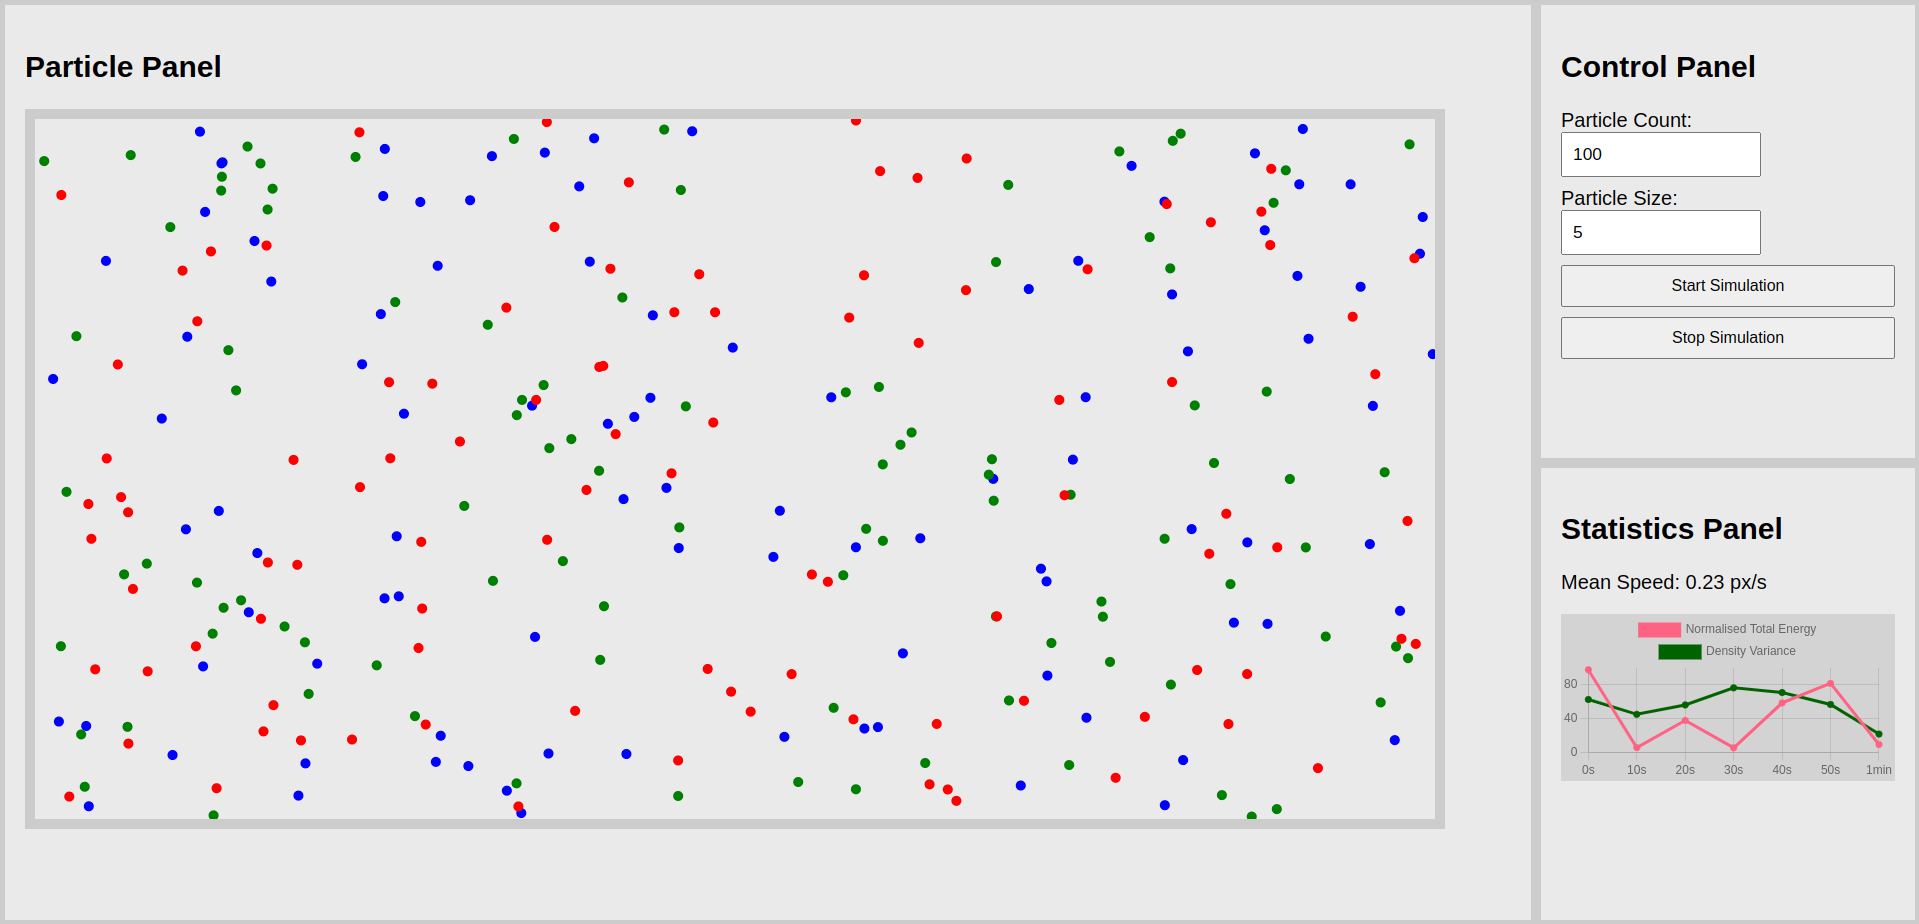
\includegraphics[width=1\linewidth]{interface/interface.png}
    \caption{Idée de l'UI}
    \label{fig:Interface1}
\end{figure}
\section{Scénarios}
\subsection{Scénario 2 familles}
\textbf{Choix :}
\begin{itemize}
    \item Deux familles (bleue et rouge),
    \item 30 particules pour la famille bleue,
    \item 15 pour la rouge,
    \item pas de relation de bleu sur rouge,
    \item relation de puissance 15 de rouge sur bleu,
    \item positionnement aléatoire.
\end{itemize}
\indent\textbf{Résultat :} \\
15 particules rouge positionnées aléatoirement, idem pour les bleues. Les bleues se rapproche petit à petit des rouges. Les rouges ne bougent pas.

\newpage
\subsection{Scénario pause/ralenti/accéléré}
\textbf{Actions :} \\
Mise en pause, puis résumé, puis ralenti et puis accéléré. \\
\indent\textbf{Résultat :} \\
La simulation se met en pause, puis repart puis ralenti puis revient à un rythme normal.

\subsection{Scénario sauvegarde}
\textbf{Actions :} \\
Sauvegarde, puis fermeture de l'application puis ouverture et enfin chargement de la sauvegarde. \\
\indent\textbf{Résultat :} \\
La simulation revient exactement au même stade que lors de la sauvegarde.

\subsection{Scénario déplacement souris}
\textbf{Actions :} \\
Appui sur le bouton gauche de la souris sur une particule puis translation à un autre endroit de la simulation et enfin relâche du bouton.\\
\indent\textbf{Résultat :}\\
La particule suit la souris jusqu'au relâchement.
\end{document}
